\section{Advanced Welding Test}

\subsection{Purpose and Focus of the Test}
The purpose of the \iaterm{Advanced Welding Test}{AWT} is to welding in two Dimensions. 
\par
The focus is on the precision required to perform a correct welding task. The detection of where to weld and the correct motion following the line, while keeping a constant movement are the keys to a successful full completion of the task. 

\subsection{Scenario Environment}
The arena used for this test contains basically all elements as for the Basic Navigation Test. Additionally to environmental elements (walls, service areas, floor markers, etc.), an object with a contour on a flat surface (see Fig. \ref{awt_examplecontour}) will be added on one or more service areas. 

\begin{figure}
\begin{center}
\subfloat[]{
\includegraphics[width = \textwidth/3]{../images/AWT_Corner.png}}
\subfloat[]{
\includegraphics[width = \textwidth/3]{../images/AWT_Curve.png}} 
\subfloat[]{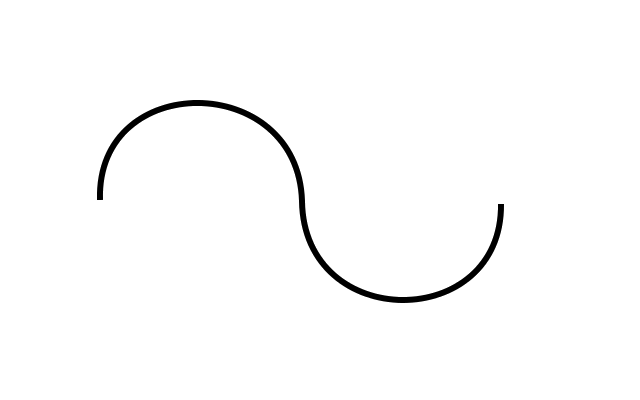
\includegraphics[width = \textwidth/3]{../images/AWT_Sinus.png}}  
\end{center}

\caption{Examples of Contours to be welded.}
\label{awt_examplecontour}
\end{figure}


\subsection{Task}
A single robot is used. The robot starts at the defined start position outside the arena. The task consists of navigating to the specified location and then welding along the defined contour. The task is finished once the contour is welded ant the robot has exited through the designated exit.
\par
The task specification consists of: 
\begin{itemize}
	\item The specification of the welding place or places (e.g. D0, S5)
	\item The specification of a final place for the robot.
\end{itemize}

Two examples for a full task specification is as follows:
\begin{itemize}
	\item AWT\textless S1,S7\textgreater 
\end{itemize}


\subsection{Complexity Options}

So far no complexity objections exist.

\subsection{Rules}
The following rules have to be obeyed:

\begin{itemize}
\item The order in which the teams have to perform will be determined by a draw.
\item A team has a time period defined int the instance specification.
\item At the beginning of a team’s period, the team will get the task specification. 
\item The team must start at in the designated start area.
\item The laser used for the test must be of or below class 1 (according to IEC 60825)
\end{itemize}


\subsection{Scoring}
Points are awarded as follows:

A System will be introduced by the TC, that allows for Measuring the distance between the contour and the welded path. If the System allows for measuring the time spent at each part and the amount of attempts used they although can be scored. All points which are closer to a point on the counter then one cm count all correct, all other points are incorrect.
\par
To allow for scoring the contour will be represented by points at corners every one cm.

\begin{itemize}
\item 5 points are awarded for every percent of the contour or contours successfully welded.
\item -100 points for every point (clustered with 1 cm diameter) outside of the contour

\end{itemize}

